\begin{frame}{\aa}{\aac}
    Supply of crop $j$ for a price $p_j$ grown by farmer $i$ is considered to depend on the willingness of the agent to supply crops at a given price:
    \begin{equation}
      S_i(p_j) = A + c_i \cdot p_j
    \end{equation}
  Here $c_i$ is the willingness to supply crop $j$  at a given price $p_j$ by farmer $i$ and $A$ is the surplus or his willingness to supply crops for free.
\end{frame}

\begin{frame}{\aa}{\aac}
Demand is considered to be a function of the population growth and the price:
  \begin{equation}
    D_j(p_j) = \left( D_0 + at^2 \right) e^{-\alpha (p_j-p_{j0})}
  \end{equation}
Where $D_0$ is a base demand, $at^2$ is a term representing population (and demand) growth as a function of time $t$, $p_j$ is the price of crop $j$ at time $t$, $p_{j,0}$ is the base price of crop $j$, and $\alpha$ is a demand slope, representing the fact that less and less people will be able to afford expensive crops.
\end{frame}

\begin{frame}{\aa}{\aac}
    \begin{columns}
      \column{0.5\linewidth}
      \resizebox{\linewidth}{!}{\begin{tikzpicture}
          \pgfplotsset{
              scale only axis,
          }
          %axis options:
          \begin{axis}[
            xlabel=Time step (years),
            ylabel=Demand for different crops,
            xmin=0,
            xmax=30,
            legend pos=south east,
            cycle list name=cropslist
          ]
            %plot 1: farmer ID 1
            \addplot+[] 
                table[y index =1]{\demandc};
            \addlegendentry{$1$}
            
            %plot 2: farmer ID 2
            \addplot+[]  table[y index =2]{\demandc};
            \addlegendentry{$2$}
    
            %plot 3: farmer ID 3
            \addplot+[] table[y index =3]{\demandc};
            \addlegendentry{$3$}
    
            %plot 4: farmer ID 4
            \addplot+[] table[y index =4]{\demandc};
            \addlegendentry{$4$}
    
          \end{axis}
        \end{tikzpicture}
      }
      \column{0.5\linewidth}
      \resizebox{\linewidth}{!}{\begin{tikzpicture}
          \pgfplotsset{
              scale only axis,
          }
          %axis options:
          \begin{axis}[
            xlabel=Time step (years),
            ylabel=Supply for different crops,
            xmin=0,
            xmax=30,
            legend pos=south east,
            cycle list name=cropslist
          ]
            %plot 1: farmer ID 1
            \addplot+[] 
                table[y index =1]{\supplyc};
            \addlegendentry{$1$}
            
            %plot 2: farmer ID 2
            \addplot+[]  table[y index =2]{\supplyc};
            \addlegendentry{$2$}
    
            %plot 3: farmer ID 3
            \addplot+[] table[y index =3]{\supplyc};
            \addlegendentry{$3$}
    
            %plot 4: farmer ID 4
            \addplot+[] table[y index =4]{\supplyc};
            \addlegendentry{$4$}
    
          \end{axis}
        \end{tikzpicture}
        }
    \end{columns}
  \end{frame}

  \begin{frame}{\ba}{\baa}
    \begin{columns}
      \column{0.65\linewidth}
      \centering
        \begin{figure}
         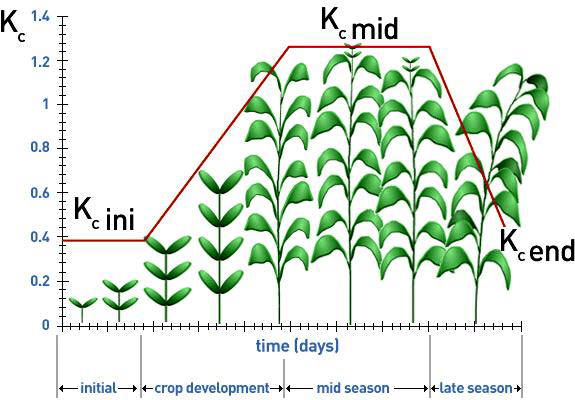
\includegraphics[width=\textwidth]{Figures/Crop-coefficients-Kc-and-growing-period-of-tomato-source-Allen-et-al-1998.png}
         \label{fig:y equals x}
        \end{figure}
        \column{0.4\linewidth}
        comment
    \end{columns}
\end{frame}

\begin{frame}{\ba}{\baa}
  \begin{columns}
    \column{0.6\linewidth}
  \begin{figure}
    \centering
    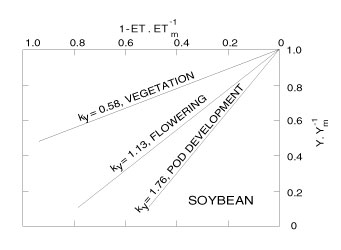
\includegraphics[width=\textwidth]{Figures/Y3655E01.jpeg}
  \end{figure}
  \column{0.4\linewidth}
  \begin{equation}
    1-\frac{Y_t^c}{Y^{m.c}}=\sum_{i=1}^{n} k_{y.i} \cdot(1-\frac{ET_{a.t}^c}{ET_{m.i}}) 
  \end{equation}
\end{columns} 
\end{frame}

\subsubsection{\bab}

\begin{frame}{\ba}{\bab}
  \begin{figure}
    \centering
    \includegraphics[width=.5\textwidth]{Figures/Emissions-by-sector-–-pie-charts.png}
  \end{figure} 
\end{frame}


\begin{frame}{\ba}{\bab}
  \begin{figure}
    \centering
    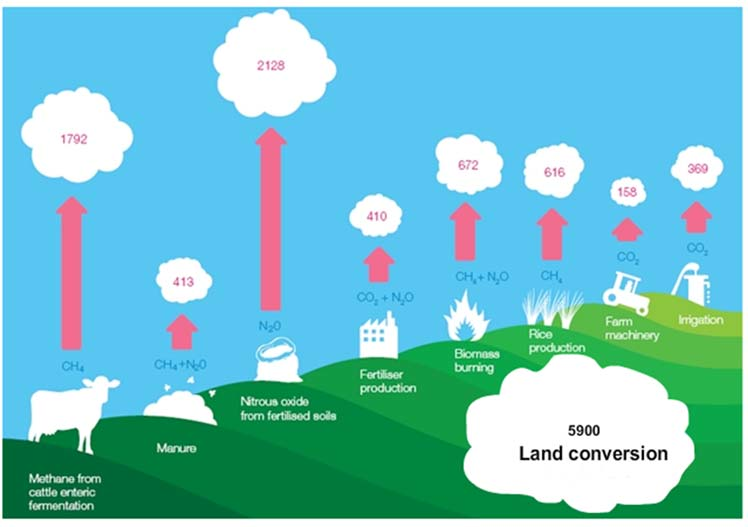
\includegraphics[width=.6\textwidth]{Figures/GHG-emissions-from-agricultural-sector-by-practices-in-Mt-CO2-e}
  \end{figure}
  \begin{equation}
    GWP_{t}=GWP_{fertilizer}+GWP_{biocide}+GWP_{machinery}+GWP_{electricity}  
    \end{equation}
\end{frame}

\begin{frame}{\aa}{\aab}
    \begin{columns}
      \column{0.48\linewidth}
      \centering
      \begin{figure}
        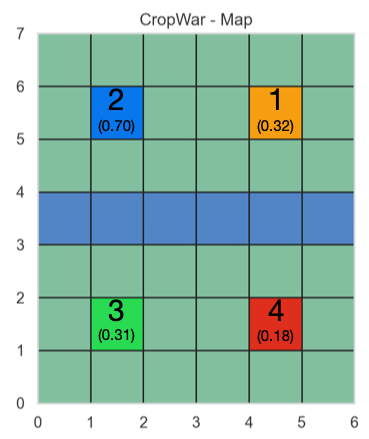
\includegraphics[width=.8\textwidth]{Figures/v12_Map_start.png}
       \end{figure}
      \column{0.52\linewidth}
      \centering
      \animategraphics[loop,width=5.8cm]{1}{Figures/V12mapGIF/frame_}{00}{10}
    \end{columns}
  \end{frame}






  \begin{frame}{\ab}{\abb}
    \begin{equation}
      \hat{g} = \hat{\mathbf{E}}_t \left[ \nabla_{\theta} \log(\pi_{\theta}(a_t|s_t)) \hat{A_t} \right]
    \end{equation}
    This would increase the probability of taking the same action decision in the same or similar state. Vice versa, the gradient is negative if the advantage is negative, which reduces the probability of taking the corresponding action.
    \end{frame}